\chapter{Introduction}
\label{chapter:intro}

\footnotesize
\indent \textbf{\textit{Summary.}} Time-memory tradeoff attacks were first conceived on block ciphers by Hellman in 1980. In this approach, Hellman proposed a method for carrying out the precomputation phase of the attack i.e. computing the precomputation tables. We refer to these tables as Hellman tables for block ciphers, in the remainder of the thesis. The proposed idea is based on the birthday paradox, and is thus probabilistic in nature, as we shall see in a moment. 

Later, using this approach as the basis, Shamir and Biryukov proposed a table structure for stream ciphers. This takes into account the amount of keystream available for the attack. We call these tables as Hellman tables for stream ciphers. We start by explaining the original idea of Hellman based on block ciphers. This is done by first presenting a naive approach to building tables for time-memory tradeoff attacks on block ciphers. Then, we point out limitations to the approach and explain how they are improved, consequently leading to the original idea of Hellman. From there, we provide the idea of Shamir and Biryukov, which is used for implementing a time-memory-data tradeoff attack on HiTag2 cipher.

\normalsize

\section{Cryptography}

Cryptography is the mathematical science of protecting secret information by transforming it into a form which is illegible. Generally, the original information is called \textit{plaintext} while the transformed information is called \textit{ciphertext}. Once plaintext is transformed into ciphertext, the latter can then be sent over an insecure channel to its destination. At the destination, the reverse transformation takes place yielding back the original information. Transformation of plaintext to ciphertext is referred to as \textit{encryption}, while the reverse process is called \textit{decryption}. A secret information called \textit{key} is used in both encryption and decryption. The key can be compared with the key for locks used to keep items safe. If the key is lost, then the lock can be broken by the holder of the key and the item can be stolen. Similarly, if an attacker knows the cryptographic key he can know the plaintext by decrypting the ciphertext.  

This is just one application of cryptography in modern security systems, namely providing confidentiality to secret information; though it was this application with which the idea of cryptography was first conceived. Modern cryptography is also capable of providing message integrity (that a message has not been modified), authentication between two parties (the guarantee that we are talking with the expected party), non-repudiation (that a party cannot deny the fact that it has carried through a transaction, if it has really done so) and so on. 

In the late 19th century, Kerckhoff published a very important principle \cite{kerckhoff} which has become the basis of modern security systems using cryptography. He said that the security of a cryptographic encryption-decryption algorithm must rest solely in the secrecy of its key, not in the secrecy of the algorithm itself. In other words, while designing a security system with cryptography, all cryptographic algorithms must be openly published, while the only secret parameter should be the keys used by the algorithms. This helps in the cryptanalysis of the algorithms and weaknesses can be found out by researchers and cryptanalysts. Though this is a very important principle, still the design of security systems continue to be based on propreitary algorithms. More information on certain secret algorithms and successful reverse-engineering techniques is provided in section \ref{sec:hitag2-background}.

Two kinds of cryptosystems exist, depending on the manner in which keys are used: symmetric-key and asymmetric-key. In symmetric-key cryptography, a single key is shared between two communicating parties, such that one party encrypts plaintext using the shared key and the other party decrypts the received ciphertext using the same key. In such systems, the secrecy of the shared key becomes extremely critical. Also, if the number of parties grows, the number of keys required in the system becomes large, since each communicating pair would hold a different key. In addition, sharing keys between each pair requires secure key establishment protocols. 

Symmetric-key cryptography was the only known kind of encryption before 1976, when Diffie and Hellman introduced the concept of asymmetric-key cryptography \cite{diffie1976ndc} for the first time. In asymmetric-key cryptography, the encryption and corresponding decryption are performed with different keys. Every party holds two keys: one public and one private. If \emph{Alice} wants to send a message to \emph{Bob}, she will encrypt the plaintext with the public key of \emph{Bob}. At the other end, \emph{Bob} would decrypt this ciphertext using his private key. The public-private key pair are related, but it is unfeasible to determine \emph{Bob}'s private key from his public key. Since every party holds two keys, the total number of keys is reduced considerably when compared to symmetric-key cryptosystems. Also, no key establishment protocols are needed as the public keys are distributed through public channels.

Symmetric-key algorithms are further classified into two different types, based on the manner in which plaintext is used by the encryption algorithm. These are block ciphers and stream ciphers. Block ciphers divide the plaintext into blocks of data, and each block is then encrypted separately. The sizes of the input and output blocks are same, irrespective of the size of the key. Successive output blocks are then connected to each other in some way, depending on the mode of operation of the block cipher. \emph{DES} (data encryption standard) has been one of the most widely used block ciphers with block size of 64 bits and key size of 56 bits. \emph{DES} has been recently replaced by \emph{AES} (advanced encryption standard) as the approved standard, through a public competition which called for new block cipher designs to replace \emph{DES}.

Stream ciphers on the other hand, have a different functional structure and working. Stream ciphers consist of an internal state, which is used in deriving one output bit through an output function. The internal state changes over successive clock cycles using an update function, consequently producing a stream of bits at the output. Bits of the plaintext are picked up in sequence and then \emph{xor}'ed bitwise with the output bits of the stream cipher to produce the ciphertext bits. The working of stream ciphers is explained in much detail in section \ref{sec:stream-cipher}. 

\section{Stream cipher}
\label{sec:stream-cipher}

\subsection{One-time pads} 
\label{sec:one-time-pads}

Before we explain the working of stream ciphers, it is important that we understand the motivation for the design of stream ciphers. An inspiration behind practical stream ciphers of today has been the one-time pad, which is also known as the Vernam cipher. In the one-time pad, the length of the key is required to be equal to or greater than the length of the plaintext. Each plaintext bit is operated with the corresponding key bit using the \emph{exclusive-or} (or \emph{xor}) operation, thus resulting in one bit of the ciphertext. So, if $p_i$ represents the $i^{th}$ bit of the plaintext, and $k_i$ represents the $i^{th}$ bit of the key, then the $i^{th}$ bit of the ciphertext is given by $c_i$ = $p_i \oplus k_i$. The corresponding decryption takes place as $p_i$ = $c_i \oplus k_i$. This is shown in the figure \ref{fig:one-time-pad}.

\begin{figure}[ht!]
	\centering
		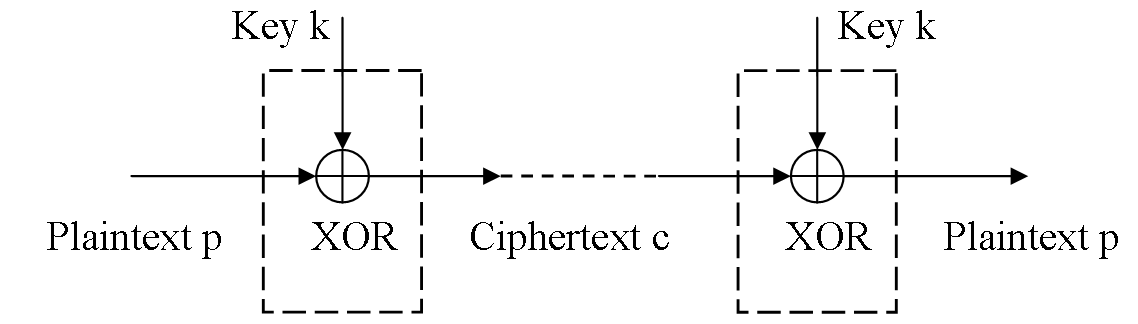
\includegraphics[width=4.4in]{./figures/one-time-pad.PNG}
	\caption{One-time pads}	
	\label{fig:one-time-pad}
\end{figure}

The key bits are required to be completely random, without any statistical correlation between them. With this pre-condition, there is no way that an adversary could determine the secret key just by knowing the ciphertext. Since the key bits are derived from a truly random source, there could be several combinations of the plaintext and the key which result in the given ciphertext. The attacker would, in such a scenario, never be able to determine which of the specific combination is the right one, even with infinite computing power at hand \cite{one-time-pads-link}.

If the attacker knows certain bits of the plaintext, then the corresponding bits of the key can be determined. If the key is not truly random, the attacker can predict some of the remaining bits of the key and thus decipher the remaining plaintext. Hence, the key should be truly random. 

Shannon in 1949, used his notion of information theory to formally prove that one-time pads are unbreakable \cite{shannon1949cts}, and termed them as having perfect secrecy. But for practical purposes, one-time pads have several weaknesses. These are explained in the following two points.
\begin{itemize}
\item The length of the key has to be equal to the length of the plaintext so that all the plaintext bits are encrypted. Thus to encrypt a long plaintext, large number of `random' key bits need to be generated. Managing such a huge set of key bits is not practical, since the storage and transfer need to be carried out securely. 

\item As the name of one-time pad suggests, a key can be used for just one transaction. If the same key is used for encrypting two different plaintext messages, the chances that the key being broken are extremely high. These chances are precisely zero when the key is used just for one encryption and is derived from a true random source. So it is suggested that a previous key not be used again.
\end{itemize}

Considering the above points, rather than transmitting the key then, it is a better idea to transmit the plaintext itself through the secure channel. Clearly, one-time pads are not good enough for being deployed in practical systems, but they reveal a strong design basis for stream ciphers. The component missing between one-time pads and stream ciphers is the pseudo-random sequence generator, which is discussed next. 

% still, one-time pad is useful. explain. 

\subsection{Pseudo-random sequence generators}
\label{sec:psrg}

Pseudo-random sequence generator (PRSG) is used to derive a seemingly random sequence of bits called the \emph{keystream}, using a small initial seed value. PRSG's are finite state machines having an internal state, which is initialized using the secret key, along with some more initialization parameters if required. A PRSG uses the following two functions internally.
\begin{itemize}
\item A linear \emph{update function} is used to derive the next state using the current state.
\item A linear or non-linear \emph{output function} is used to generate an output bit from the current state. 
\end{itemize}

\begin{figure}[ht!]
	\centering
		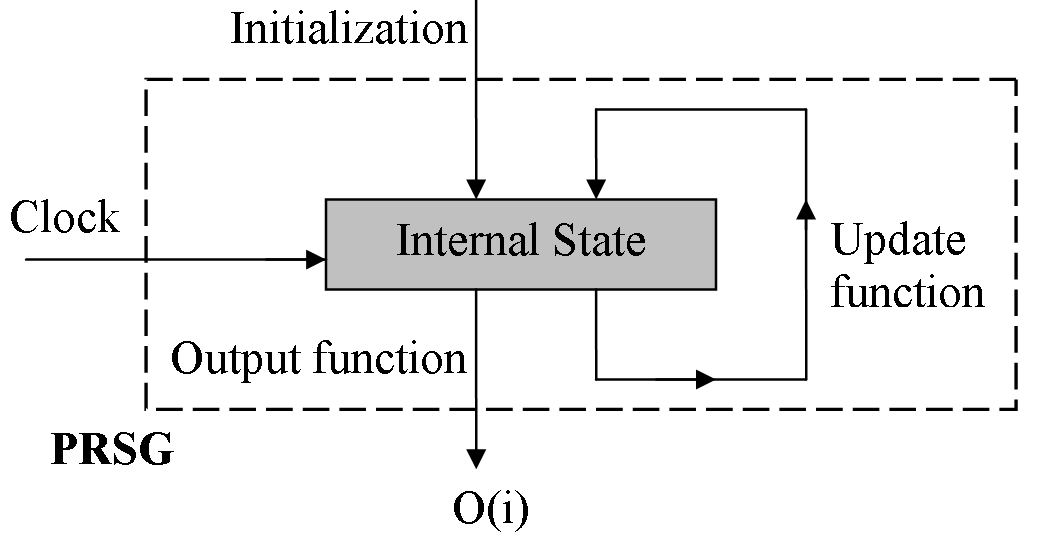
\includegraphics[width=3.5in]{./figures/prsg.PNG}
	\caption{Internal model of Pseudo-random sequence generator}	
	\label{fig:prsg}
\end{figure}

Figure \ref{fig:prsg} shows the internal model of a PRSG. A stream of the output bits (occuring as the PRSG changes states in every clock cycle) constitutes the keystream. It is important to note that the keystream is not truly random, but as the name of the generator suggests, it is pseudo or seemingly random. 

\paragraph{\textit{Use in stream cipher construction.}}
\label{para:stream-construction} 
We need to use secret keys of fixed length independent of the length of plaintext, in the construction of stream ciphers. Typically the key lengths are 128, 256 or 512 bits, which are considered secure by the standards of the computational power existing today. 
% NEEDED - check this and need a reference here %
The small secret key is used in the initialization of the PRSG thus generating a long keystream which replaces the long secret key in the one-time pads. The trade-off here is that the keystream is not truly random. As a result, the perfect secrecy of one-time pads does not apply to stream ciphers, but at the same time, the strength of the pseudo-random sequence generator becomes extremely important in determining how strong the stream cipher is cryptographically.

An overview of a stream cipher design is shown in figure \ref{fig:stream-cipher}. The secret key and other initialization parameters like initialization vector (IV) etc. are used to initialize the internal state. Once the initial state is prepared, the PRSG is ready to generate the keystream. Bits of the plaintext are \emph{xor}'ed along with corresponding bits from the keystream to generate a stream of encrypted bits. In effect, the plaintext and the keystream are used to produce the ciphertext.

\begin{figure}[ht!]
	\centering
		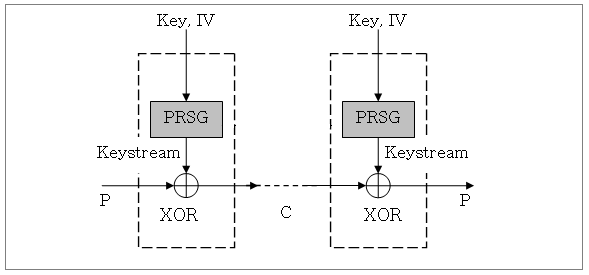
\includegraphics[width=4in]{./figures/stream-cipher.PNG}
	\caption{Deployment of PRSG in a stream cipher}	
	\label{fig:stream-cipher}
\end{figure}

At the receiver end, the PRSG is initialized using the same parameters. Any change in the initialization results in the generation of a different keystream leading to incorrect decryption of the received ciphertext. With the correct keystream, ciphertext is decrypted giving the correct plaintext. 

% security of PRSG %
As briefly mentioned before, the security of the stream cipher much depends on the security properties of PRSG. The output sequence is required to behave as a true random sequence. One very important consideration in ascertaining adequate security \cite{robshaw1995sct} is mentioned below.

The period of the keystream should be large. This becomes extremely important when the length of the plaintext is large. If the keystream repeats, the same sequence would encrypt different parts of the plaintext. If the attacker has knowledge of some initial part of the plaintext, then the initial keystream encrypting the known plaintext can be recovered. This initial keystream can later be used to decrypt part of the ciphertext which the attacker does not know. Even if the attacker has no knowledge of plaintext, certain properties of the plaintext can be derived from the two ciphertexts encrypted using the same keystream. 

On the other hand, the requirement on how large the period should be depends on the amount plaintext expected to be encrypted.

\subsection{Linear feedback shift registers} 
\label{sec:lfsr}
The most widespread implementation of PRSG's is done using a linear feedback shift register (LFSR). Other methods for generating pseudo-random sequences exist as well. Since we are mainly going to deal with an LFSR based generator (HiTag2) in this thesis, we would describe only them here. Other methods of generating pseudo-random sequences are linear congruence generators and non-linear feedback shift registers. For an introduction to these methods, we point to \cite{zeng1991pbg}. 
% reason why LFSR are widely used, and why are we more interested in them %
% more info on other generators %

It is important to note that LFSR constitutes only the \emph{update function} of the PRSG. The \emph{output function} of the PRSG needs to be implemented on top of the LFSR. An LFSR consists of two important components which are a shift register and a linear feedback function.\\

\textbf{\emph{Shift Register.}} A shift register holds a fixed number of bits, and shifts each of them into corresponding adjacent positions (all in a particular direction) on every clock cycle. If the direction of the shift is taken to be rightwards, then in every clock cycle there is a new bit on the leftmost position of the register, and the rightmost bit is excluded from the register, as shown in the figure \ref{fig:shift-register}. If the $n$ bits of the shift register are represented by $s_{n-1}$, $s_{n-2}$, $\ldots$ , $s_{1}$, $s_{0}$, then on every clock cycle we have the following transformations: $s_{out}$ = $s_{0}$, $s_{0}$ = $s_{1}$, $\ldots$, $s_{n-2}$ = $s_{n-1}$, $s_{n-1}$ = $s_{in}$; where $s_{out}$ is the bit which is excluded from the register and $s_{in}$ is the new bit. The application implementing the shift register decides how the $s_{in}$ and $s_{out}$ bits are handled.

\begin{figure}[ht!]
	\centering
		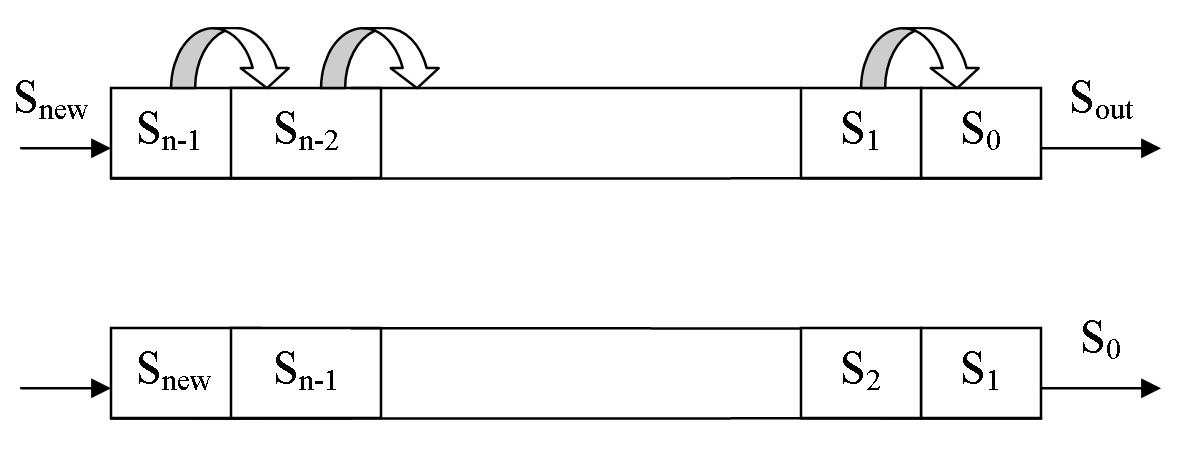
\includegraphics[width=4in]{./figures/shift-register.PNG}
	\caption{A simple shift register and its state after one clock cycle}	
	\label{fig:shift-register}
\end{figure}

For example, one of the uses of shift registers has been in the conversion of sequential (or serial) data to parallel data, and vice versa \cite{lfsr-link}. A sequence of bits can be stored in the shift register over a period of $n$ clock cycles, and retrieved in a parallel form in the $(n+1)$'th clock cycle. Hence, $s_{in}$ bit is taken from the input sequential stream, while $s_{out}$ bit is not used. 

For parallel-to-sequential data conversion, a parallel stream of $n$ bits is stored in the shift register in one cycle, and retrieved sequentially over the next $n$ clock cycles. The bit $s_{in}$ is not used in this case and $s_{out}$ stores bits of the sequential output stream.\\

\textbf{\emph{Linear feedback.}} A \textit{feedback function} defines the $s_{in}$ bit as a function of one or more bits from among the $n$ bits of the shift register. If the function is \textit{linear}, it said to be a \textit{linear feedback function}. Linearity is incorporated in the design generally by the use of $xor$ as the feedback function. Other boolean functions which are linear are negation, logical biconditional, tautology, and contradiction. According to the Wikipedia page on linearity \cite{linear-wiki}, 
\begin{quote}
\footnotesize{A Boolean function is linear if (1) In every row of the truth table in which the value of the function is `T', there are an even number of `T's assigned to the arguments of the function; and in every row in which the truth value of the function is `F', there are an odd number of `T's assigned to arguments; or (2) In every row in which the truth value of the function is `T', there are an odd number of `T's assigned to the arguments and in every row in which the function is `F' there is an even number of `T's assigned to arguments.
}
\end{quote}

The above properties can be easily checked to hold in the truth table of the \emph{xor} function.

A simple example of an LFSR is shown in figure \ref{fig:lfsr-example1}. Let us examine the linear feedback function more closely for this example. As can be seen, certain selected bits from the shift register are \emph{xor}'ed, and the resulting value is assigned to the leftmost bit, but only in the next clock cycle (in addition to the shifting of bits). As a result, the internal state of the LFSR is changed. If we number the bits from \emph{1, 2,} $\ldots$ , and so on, then the bits 11, 13, 14 and 16 are used in the feedback function. These bits are referred to as \emph{tap sequence} or $taps$ of the LFSR. In general, the outputs that affect the input of the LFSR are called $taps$.\\


\begin{figure}[ht!]
	\centering
		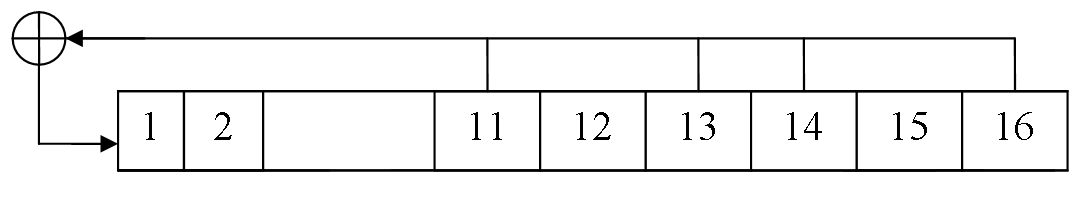
\includegraphics[width=4in]{./figures/lfsr-example.PNG}
	\caption{A simple LFSR of size 16 bits and tap bits 11, 13, 14 and 16}	
	\label{fig:lfsr-example1}
\end{figure}

\noindent \textit{\textbf{Maximal length tap sequence.}} Depending on the initial state, the LFSR runs through a set of states and then returns back to the initial state. This forms a cycle of states. In order to use the LFSR for generating a pseudo-random sequence, we want to have the longest cycle of the LFSR states. In other words, we want the LFSR to traverse through all possible states, which is equal to $2^n$, where $n$ is the number of bits in the shift register. This is important since it is desired that the pseudo-random sequence has a large period, as mentioned in the requirements for PSRG in section \ref{para:stream-construction}.

It is important to note that if the LFSR is in a state where all the bits are \textbf{0}, then the next state would also be the same. This condition occurs because the \textit{xor} of any number of \textbf{0}'s is always \textbf{0}. Such a state is called the \textit{trivial state}. As a result, no cycle is formed if the initial state is the trivial state. Hence the maximum number of different states in the LFSR becomes $2^n-1$. A tap sequence which generates the particular cycle of states such that the period of the LFSR is $2^n-1$, is called the maximal length tap sequence. 

The tap sequence for the LFSR in figure \ref{fig:lfsr-example1} is a maximal length tap sequence. In order to verify maximal length tap sequences, the polynomial representation of the tap sequence is considered.\\

\noindent \textit{\textbf{Polynomial representation of tap sequence.}} Once we have a tap sequence, we can express it in the form of a polynomial with modular \textbf{2} coefficients. For the example shown in figure \ref{fig:lfsr-example1}, the polynomial representation of the tap sequence is

\begin{center}
$p(x)$ =  1 + $x^{11}$ + $x^{13}$ + $x^{14}$ + $x^{16}$
\end{center}

The powers of $x$ represent the tap bits. The \textbf{1} in the starting is a result of $x^0$ and represents the $s_{in}$ bit, since $s_{in}$ can be interpreted to exist at the \textbf{0}'th position of the shift register (this existence is just theoretical). A given tap sequence is a maximal length tap sequence if the polynomial representing it is irreducible i.e. the polynomial cannot be factored into nontrivial polynomials.

It is important to note that the polynomial representation should not depend on the numbering of the bit positions. If the same LFSR is numbered in the fashion as shown in figure \ref{fig:lfsr-example2}, then we have the following polynomial representation.

\begin{align*}
p'(x) &= x^{17} + x^{6} + x^{4} + x^{3} + x
\end{align*}

\begin{align}
\label{eq:poly-1} p'(x) &= x*(x^{16} + x^{5} + x^{3} + x^{2} + 1)\\
\label{eq:poly-2} p'(x) &= x^{16} + x^{5} + x^{3} + x^{2} + 1
\end{align}


\begin{figure}[ht!]
	\centering
		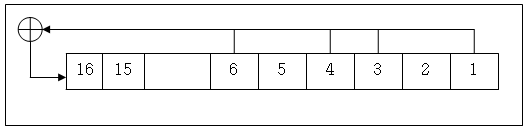
\includegraphics[width=4in]{./figures/lfsr-example-reverse.PNG}
	\caption{A different numbering of the bit positions for the same LFSR}	
	\label{fig:lfsr-example2}
\end{figure}

The ploynomial in equation \ref{eq:poly-1} is irreducible only if the term $(x^{16} + x^{5} + x^{3} + x^{2} + 1)$ is irreducible, so we rewrite $p'(x)$ after ignoring the factor $x$ in the equation. Since both $p'(x)$ and $p(x)$ represent the same LFSR, they should be related in some way. The Wikipedia page for LFSR at \cite{lfsr-wiki} states the following in this context,

\begin{quote}
\footnotesize{
Once one maximal tap sequence has been found, another automatically follows. If the tap sequence, in an $n$ bit LFSR, is [n,A,B,C,0], where the \textbf{0} corresponds to the $x^0$ = 1 term, then the corresponding `mirror' sequence is [n,n-C,n-B,n-A,0].}
\end{quote}

In our example, the tap sequence [16,14,13,11,0] has a mirror tap sequence [16,5,3,2,0], which are represented by the polynomials $p(x)$ and $p'(x)$.

Hence, the choice of an appropriate polynomial for the LFSR is important in order to guarantee that the LFSR moves through all the possible internal states before the first state repeats.

%
% NEEDED - \subsection{Some stream ciphers}
%

\section{The HiTag2 stream cipher}
\label{sec:hitag2}

\subsection{Background}
\label{sec:hitag2-background}
HiTag2 is a stream cipher originally designed by Philips Semiconductors (now NXP Semiconductors) and used for mutual authentication between a car remote control and controller in the car. Such systems (called remote keyless entry or RKE systems) have been widely implemented in modern electronic cars, and facilitate unlocking of car doors upon just a button press from within a certain maximum distance from the car. The HiTag2 stream cipher provides two-way authentication, authenticating the two entities to each other one by one. In such a protocol, a nonce is sent across from the initiator to the responder. The responder initializes the stream cipher using the nonce as IV, additionally using the secret key and its fixed ID. Some fixed length of the keystream is then sent back to the initiator as authenticator. The similar protocol is executed to authenticate the initiator to the responder. 

But, this is just one use of the cipher, and other applications could use the cipher for authentication as well as encryption. If hiding the plaintext is desired, the message bits are \emph{xor}'ed with the keystream bits before sending them over the public channel. 

HiTag2 was kept secret by Philips until it was reverse-engineered using the cipher's software implementation. The microcode (or assembly code) of HiTag2 was decompiled from the implementation available in the car remote controls and the RKE receivers. The C code for the cipher is availabe on the website \cite{hitag2-code}. A full system level specification of the RKE system by Philips (titled Active Tag and IC) implementing the HiTag2 cipher is also available \cite{active-tag-datasheet}. HiTag2 now is the intellectual property of NXP, but the specification document holds the name of Philips since NXP did not come into existence at that time in 2005. Also, since the cryptography (HiTag2) on the RKE system was kept secret at that time, HiTag2 modes are just mentioned without any further information on the functional working of the cipher.

The design of HiTag2 is very similar to a recently reverse-engineered \cite{NohlESP-2008-usenix} stream cipher called Crypto-1, which is used in Mifare Classic smartcards by NXP. The Mifare family comprises of contactless smart cards and card readers, with a variety of different features including memory availability on the cards to store data and read/write permissions on the cards. As a result of these features, Mifare system is widely used in applications requiring more than just authentication. Some such applications are ticketing system for public transportation (OV-Chipkaart in Netherlands, Oyster cards in UK etc.) and access control in buildings. Crypto-1 cipher used in Mifare Classic cards and readers was proprietary until recently when Nohl et. al. \cite{NohlESP-2008-usenix} reverse-engineered the algorithm from its silicon implementation.

In addition, the same Mifare Classic cards and readers are shown to be easily clonable \cite{dekoninggans2008pam} by researchers at Radboud University. They have analyzed the communication protocol between the card and the reader, and have been been able to show that the there are several weaknesses in the Crypto-1 cipher. They have been able to recover the necessary keystream by analyzing the protocol messages. The details of this protocol analysis complements the work by Nohl et. al., and using both the ideas, mounting brute-force attack on the cipher has been made possible. 

Apart from reverse-engineering from software or hardware implementations, a black-box reverse-engineering has also been applied to break secret algorithms. The DST RFID tag (using the DST stream cipher) was broken in 2005 using black-box reverse-engineering \cite{bono2005sac}, i.e. by selecting certain input formats and using both the input and output combinations to deduce the structure and working of the cipher. The most common application of Texas Instrument's DST tag is in vehical immobilizer systems and electronic payment systems \cite{dst-rfid-analysis}. 

In the next section, the working of HiTag2 is described.

\subsection{Cipher Description}
The basic components of the HiTag2 stream cipher are outlined below.
\begin{itemize}
\item 48 bit key
\item 32 bit serial ID
\item 32 bit initialization vector (IV)
\item 48 bit internal state with linear update function (basically, an LFSR)
\item Non-linear output function based on multiplexor, with data bits being constant and address bits depending on the current internal state
\end{itemize}

The entire setup of the keystream generator is done in two phases. The first phase is the initialization of the LFSR, which sets the internal state to a non-zero value using the key and the serial ID. The second phase is the setup of the LFSR during which the LFSR is clocked (resulting in the shifting of bits) using the key and IV bits in the process. Once the LFSR is set, the keystream is ready to be generated from the internal state right away. We describe these phases in detail here.\\ 

\noindent \textit{\textbf{1. LFSR Initialization.}} The initialization step of the LFSR is straightforward. Instead of initializing the LFSR with random bits, the serial ID and an initial part of the key are used. The 32 bits of the serial ID are stored in the least significant 32 bits of the LFSR (bits from index 0 through index 31). Then, the least significant 16 bits of the key are stored in the remaining 16 bits of the LFSR (bits from index 32 through index 47), as shown in figure \ref{fig:hitag2-1}. With this the initialization of the LFSR is complete.\\

\begin{figure}[ht!]
	\centering
		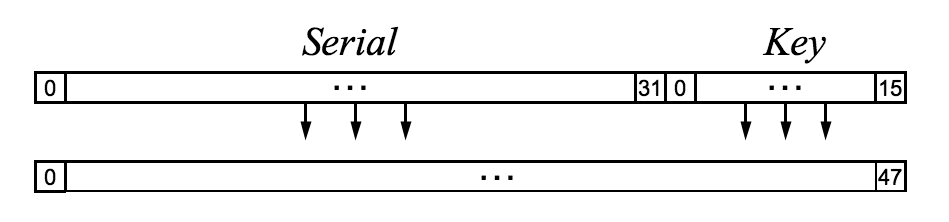
\includegraphics[width=5in]{./figures/hitag2-1.PNG}
	\caption{LFSR Initialization}	
	\label{fig:hitag2-1}
\end{figure}

\noindent \textit{\textbf{2. LFSR Setup.}} During the setup of the LFSR, the 32 bits of IV are used with the remaining 32 bits of the key. The bits in the LFSR are shifted to the right in every clock cycle, and a new value is stored in the leftmost bit. In every clock cycle, an xor of the following three bits is computed: one bit from the key (range: bits from index 16 through 47), one bit from the IV (range: bits from index 0 through 31) and the output bit from the non-linear output function. The computed bit is stored at the leftmost bit of the LFSR. After 32 clock cycles, the internal state is prepared for keystream generation. This is shown in figure \ref{fig:hitag2-2}.\\

\begin{figure}[ht!]
	\centering
		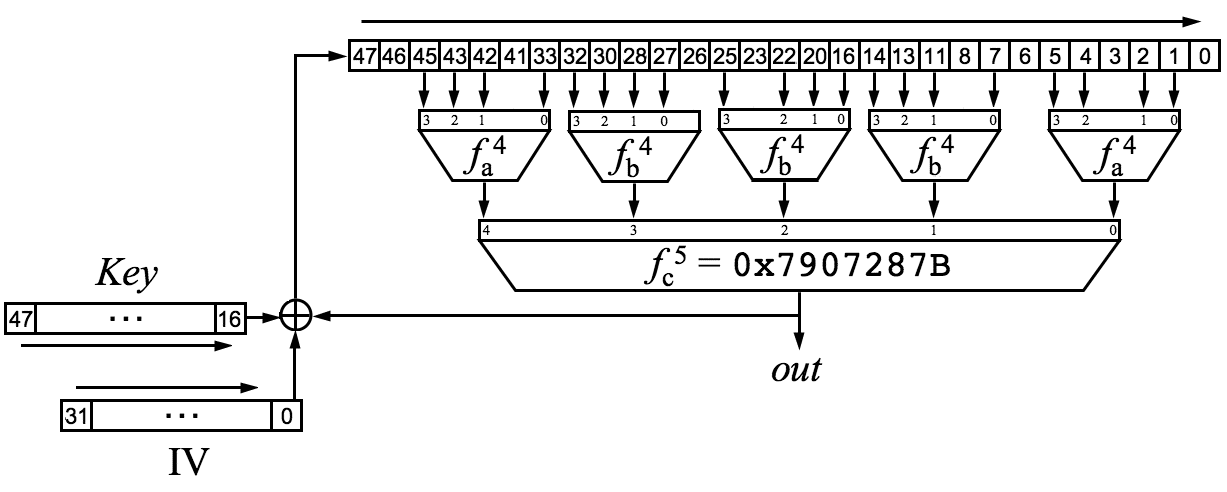
\includegraphics[width=5.5in]{./figures/hitag2-2.PNG}
	\caption{LFSR Setup Phase}	
	\label{fig:hitag2-2}
\end{figure}

\noindent \textit{\textbf{Output function.}} The output function consists of two levels of multiplexors. The multiplexors have fixed data bits, whereas the address bits are chosen either from the LFSR or from other multiplexors. In the first level, 20 bits from the LFSR are used as address bits to five four-bit multiplexors, giving a total of five bits of output (one from each multiplexor). These five bits are then used as address bits to the single five-bit multiplexor in the second level. The output bit of this multiplexor gives the stream cipher's output bit, constituting the keystream. In all, six instances of multiplexors cover the two levels of the output function.

\begin{table}[ht!]
\begin{center}
\small{
\begin{tabular}{|p{2.2cm}|l|p{2cm}|p{2.8cm}|p{1.5cm}|}
\hline 
\textbf{Multiplexor instance}	& \textbf{Function}		& \textbf{Data bits}	& \textbf{Address bits (input)}		& \textbf{Output bit}\\ \hline \hline
\multicolumn{5}{|c|}{Level 1 Multiplexors}\\ \hline \hline
MUX 1 			&	$f_a^4$			& 0x2C79			& 1, 2, 4, 5							& $o_1$\\
MUX 2 			&	$f_b^4$			& 0x6671			& 7, 11, 13, 14						& $o_2$\\
MUX 3 			&	$f_b^4$			& 0x6671			& 16, 20, 22, 25					& $o_3$\\
MUX 4 			&	$f_b^4$			& 0x6671			& 27, 28, 30, 32					& $o_4$\\
MUX 5 			&	$f_a^4$			& 0x2C79			& 33, 42, 43, 45					& $o_5$\\ \hline \hline
\multicolumn{5}{|c|}{Level 2 Multiplexor}\\ \hline \hline
MUX 6 			&	$f_c^5$			& 0x7907287B	& $o_1$, $o_2$, $o_3$, $o_4$, $o_5$		& $k_i$\\ \hline
\end{tabular}}
\end{center}
\caption{Multiplexors making the output function}
\label{tab:muxs}
\end{table}

Three different multiplexor functions are used to realize these six instances, and these are called $f_a^4$, $f_b^4$ and $f_c^5$. While $f_a^4$ and $f_b^4$ take in four bits for addressing the output, $f_c^5$ takes in five bits. The multiplexors $f_a^4$ and $f_b^4$ are used in the first level, where as $f_c^5$ is used in the second level. These six instances are described in the table \ref{tab:muxs}. In the table, the input bits for the first level of multiplexors are indicated by the index of their position in the LFSR.

It is important to note that the update function of the LFSR is not used in both the initialization and setup phases of the cipher. This function is used during the keystream generation as discussed next.\\

%The source code for the initialization and setup of the LFSR is shown below in the listing. Here, the function \emph{hitag2\_output} stands for the output function, which we have just described.\\

% NEEDED - explain a little about the implementation before the code snippet. 

%\lstinputlisting[frame=tb, caption={HiTag2 initialization code snippet}]{./code-snippets/hitag2_init.c}

\noindent \textit{\textbf{3. Keystream Generation.}} The output from the function $f_c^5$ constitutes the keystream. In addition, the LFSR state is changed in every clock cycle through the update function. The internal state is updated linearly, in the following fashion: the leftmost bit of the LFSR is replaced with the \textit{xor} of taps of the LFSR (which are bits 0, 2, 3, 6, 7, 8, 16, 22, 23, 26, 30, 41, 42, 43, 46 and 47). The remaining bits are shifted rightwards to adjacent positions. Once the internal state is changed, the output bit gets recomputed, generating the next bit of the keystream. This is shown in figure \ref{fig:hitag2-3}. 
%Following is the code snippet for the function implementing one round of the HiTag2 (\emph{hitag2\_round}), by first updating the state and then calling the output function (\emph{hitag2\_output}).\\

%\lstinputlisting[frame=tb, caption={HiTag2 keystream generation code snippet}]{./code-snippets/hitag2_round.c}

\begin{figure}[ht!]
	\centering
		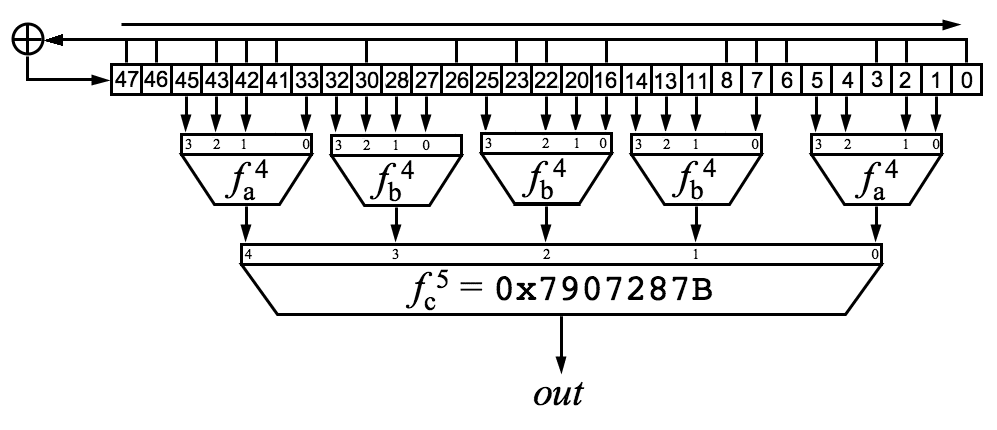
\includegraphics[width=5in]{./figures/hitag2-3.PNG}
	\caption{Keystream Generation}	
	\label{fig:hitag2-3}
\end{figure}

%\subsection{Brief security analysis}
%\label{sec:hitag2-security-analysis}
% a basic cryptanalysis of the cipher - maximal period? linearity? %
